\chapter{Evaluation}\label{c:eval}
%\begin{itemize}
%	\item Microbenchmark: Memory Allocation
%	\item Microbenchmark: Memory Migration w. NUMA Nodes
%	\item Benchmark: Example Application w. and without NUMA-aware UM
%	\item Memory Footprint Analysis
%	\item ??Interconnect Analysis?? (How is QPI-Communication influenced)
%\end{itemize}
To determine the performance impact of NUMA affinity a set of benchmarks is performed. Before an application benchmark is evaluated, a set of micro benchmarks determines specific performance metrics in order to find out how the wrapper code impacts basic performance.

The benchmarks were executed on a system with following specification:
\begin{itemize}
	\item 2 x NVidia GeForce GTX 1070 (Pascal)
	\item 2 x Intel Xeon E5504 @ 2.0GHz (Nehalem) \newline Setup as two NUMA nodes
	\item 72Gbyte DDR3 RAM (Hynix HMT151R7BFR4C-G7)
	\item OS: CentOS Linux release 7.3.1611 (Core)
	\item HWLOC 1.11.2
	\item CUDA 8.0
\end{itemize}
The physical configuration is displayed in Figure \ref{f:sys}

\section{Microbenchmarks}
\subsection{Allocation}
Because the allocation is more complicated than \verb|cudaMallocManaged|, the additional data movement
impact is analysed. Because every buffer is copied to the host for NUMA placement, the benchmark does the same
for memory allocated with \verb|cudaMallocManaged| to compare the impact.

Figure \ref{f:micro} shows that allocation using \verb|numaMallocManaged| needs multiple orders of magnitude more time compared
to \verb|cudaMallocManaged|. This is caused by the required Device-to-Host copy of all pages. To address this, a second benchmark shows the performance of \verb|cudaMallocManaged| with additional
memory migration. The data shows, that the allocation used by the NUMA wrapper is still significantly more expensive.
The reason for this is the allocations performed on all NUMA nodes and the syscalls used to query thread ids and binding threads to a 
NUMA node.
\begin{figure}[tp]
	\centering
	\begin{minipage}{0.5\textwidth}
		\centering
		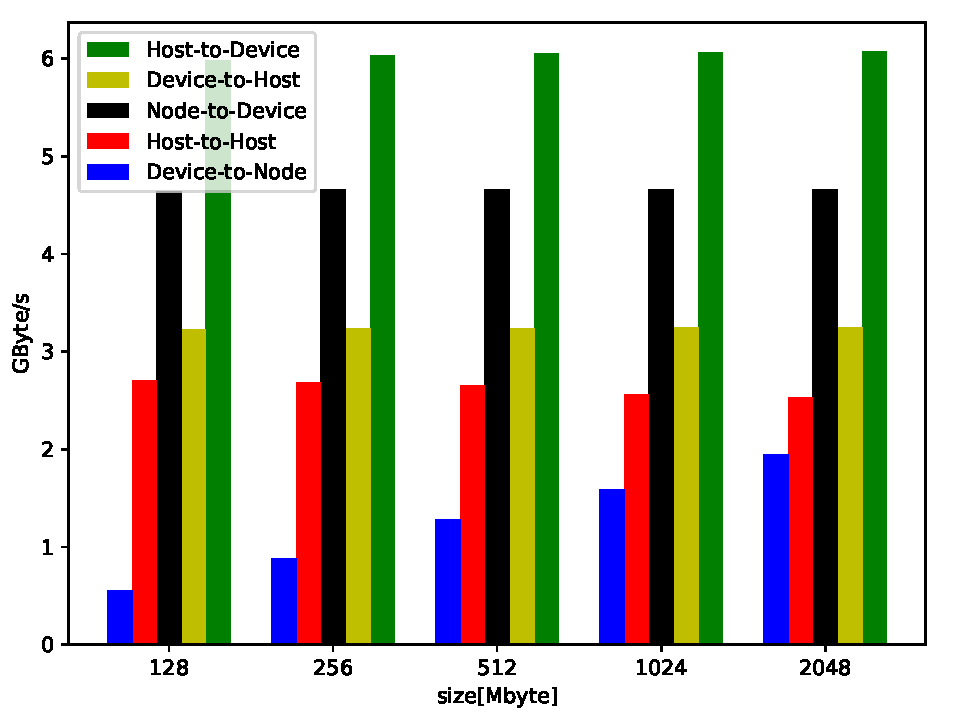
\includegraphics[width=\textwidth]{bw-plot}
	\end{minipage}\hfill
	\begin{minipage}{0.5\textwidth}
		\centering
		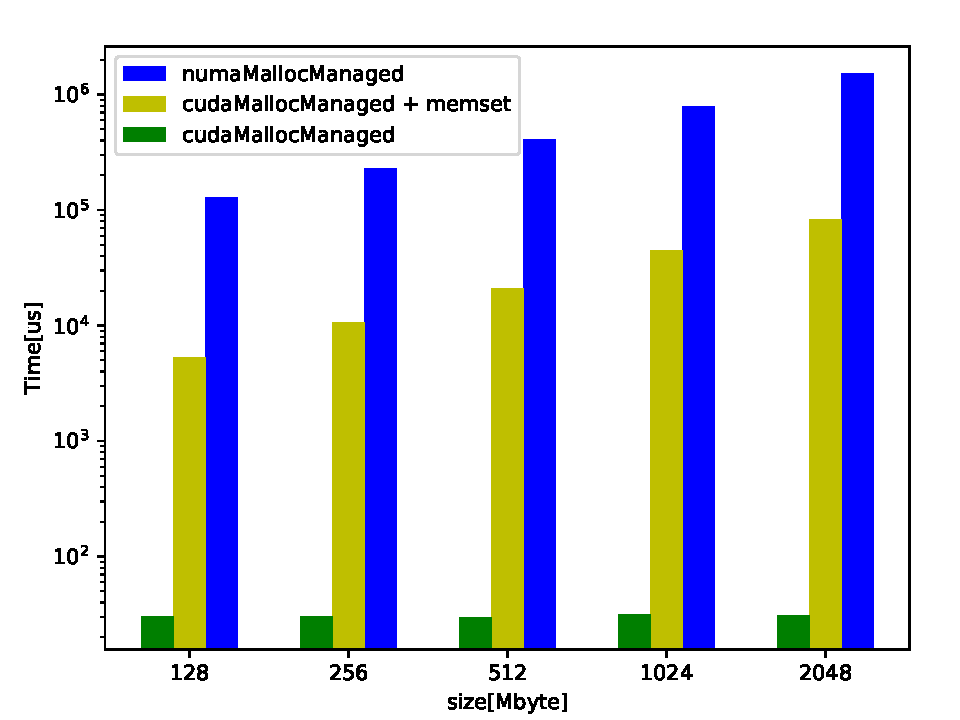
\includegraphics[width=\textwidth]{alloc-plot}
	\end{minipage}
	\caption{(L): Bandwidths achieved with the NUMA interface \newline (R): Allocation time compared between NUMA interface and CUDA interface}
	\label{f:micro}
\end{figure}
\subsection{Memory Migration}
Moving data inside the system can be the defining factor for the performance of an application. A series
of benchmarks quantifies the impact of data migration between different NUMA nodes and CUDA devices.

Figure \ref{f:micro} shows bandwidth measurements for data sets of various sizes. Both Host-to-Device and Device-to-Host
match the bandwidths achieved with CUDA (not displayed here). This means the wrapper does not reduce the performance
of already existing functionality.
Node-to-Device shows the bandwidth for transfers from NUMA nodes that are not directly connected to the device.

Host-to-host performance displays the achievable transfer bandwidth between two NUMA nodes and is depending on the used interconnect and the available memory bandwidth. The constant
performance shows that overheads caused by thread starting and joining can be neglected.

The Device-to-Node transfer shows the achievable bandwidth when copying data from a device to another NUMA node.
The achievable bandwidth is lower than a normal device-to-host transfer because twice the data needs to be moved, first
from device to the host, then to the targeted NUMA node.


\subsection{Memory Footprint}
Since memory is allocated for every NUMA node on the system, the memory footprints is multiplied by the number of NUMA nodes
in the system. The memory footprint is increased the factor that is the number of NUMA nodes in the system. 

\section{Application Benchmark}
To measure NUMA effects on an application, this benchmark runs a heterogeneous  pseudo-workload that quantifies the effects of NUMA locality for workloads that are shared between host and device. The workload performs an increment on every data element and ensures data movements are not optimized out by compilers
or the runtime and to simulate work that is performed during CPU and GPU computations.
First the benchmark performs the workload on one GPU and the NUMA node with the closest proximity. This ideal placing
serves as a reference for later runs. 
To measure the NUMA effects, the same workload is executed on the second GPU, with varying NUMA nodes. Which NUMA node the data is placed on, can be configured. This is used to measure how expensive non-optimal NUMA placement can be.

Performance is evaluated by relative increase of total execution time between first (ideal) and second run. 
The increase is the time lost due to data movement across NUMA nodes. Total time of second run includes
the time required to migrate the data to another NUMA node, if migration is performed.

Figure \ref{f:appaff} displays how performance is affected by multiple factors, for workloads that use
explicit prefetching of data between host and device.
\begin{itemize}
	\item \textbf{Size:} Size of workload.  
	\item \textbf{Kernel Runtime:} How long a single computation is performed. This is controlled by the number of workload iterations. Applied separately to CPU and GPU kernel.
	\item \textbf{Iterations:} How often CPU and GPU take turns in the computation. Increasing the parameter increases the number of times data is moved between host and device.
	\item \textbf{Affinity:} Control if data is moved to the NUMA node with the PCIe controller of the second GPU.
\end{itemize}

Generally the data in Figure \ref{f:appaff} suggest that every factor that contributes to an increased
computation runtime  mitigates the influence of NUMA migration on overall execution time, which is only depending on the size of the workload and available hardware. 

First we will look at the short running kernels (3 iterations of the workload). Here we see a spike
in the black bar for the workload of 128 MByte with no affinity and low data movement. The reason for this spike is the lower bandwidth and higher latency between host and device memory, which weigh in heavy against the very short
overall runtime. 

Since more application iterations also mean a higher compute time (3*3 iterations vs. 3*16 iterations) the effects are less visible. The blue bars dominate larger workloads because of the high
amount of traffic between host and device which is impaired by NUMA effects and small compute time in-between.

The green bar shows the best performance because it only hast to perform one Node-to-Node copy
and afterwards can benefit from the full bandwidth available between host and device. So the visible runtime increase is almost exclusive
the cost of one Node-to-Node transfer. For the yellow bar this static overhead of one data migration is larger due to a lower overall computation time, explaining the higher increase in runtime.

\begin{figure}
	\centering
	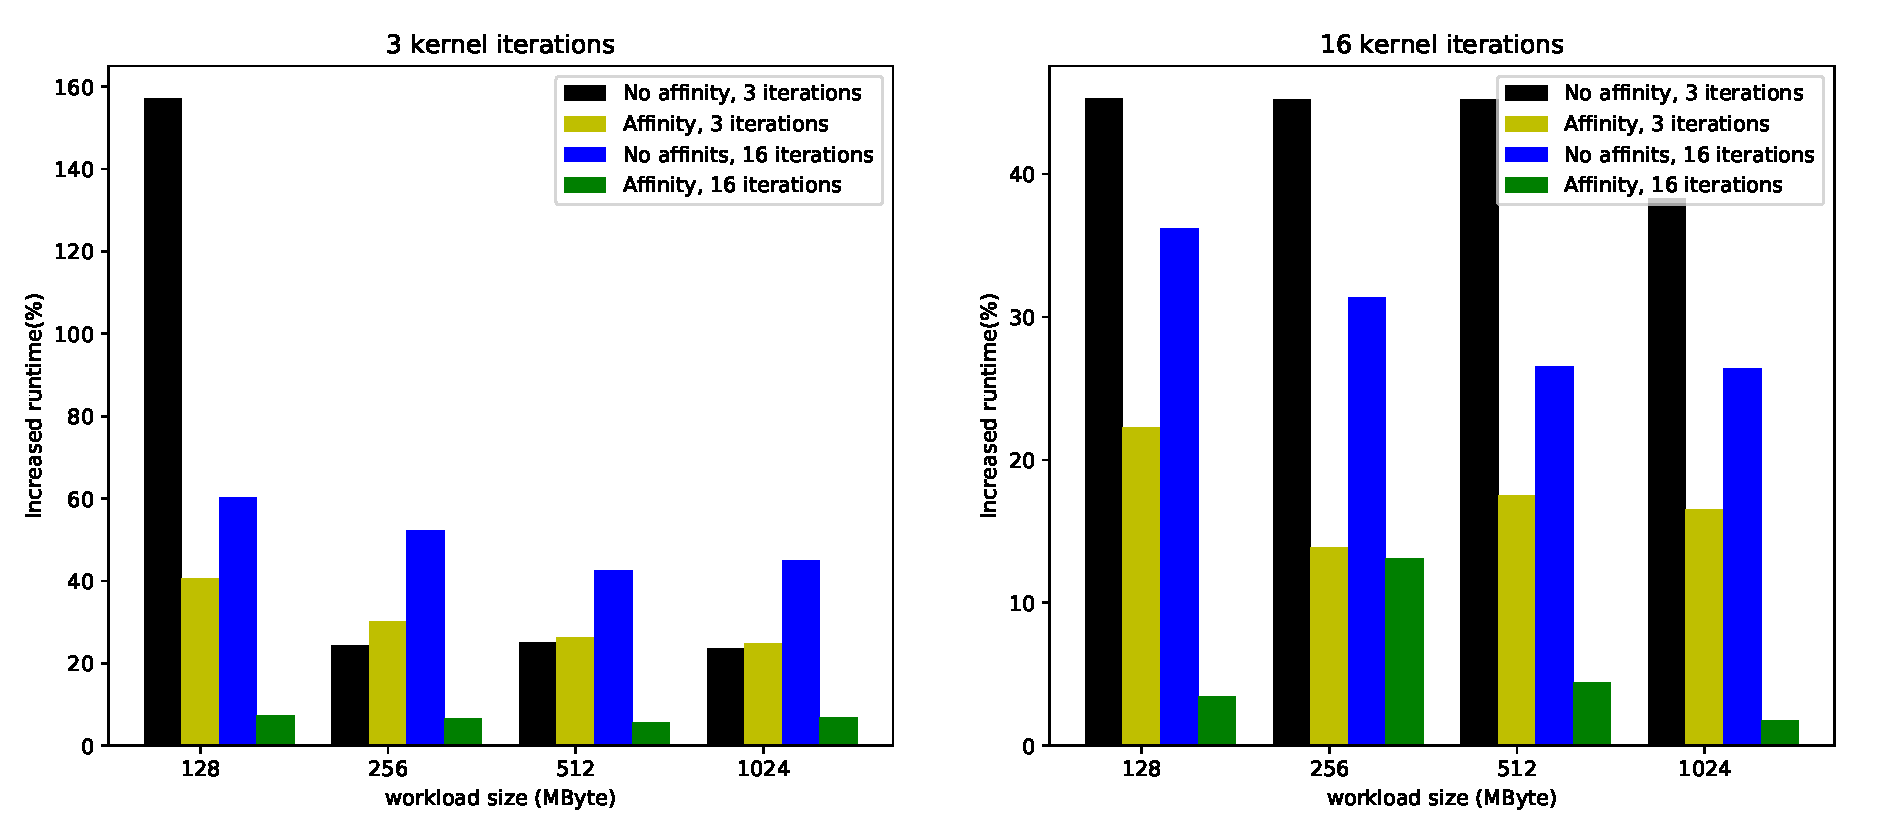
\includegraphics[width=\textwidth]{app-affinity}
	\caption{ NUMA-Effects on pseudo-workload. Displayed as increase of runtime relative to a run with ideal NUMA placement between host and device. With explicit data movement.
		The left hand side shows the relative increase in short running computational kernels.
		The right hand side shows the retlative increase on long computational kernels.}
	\label{f:appaff}
\end{figure}

\begin{figure}
	\centering
	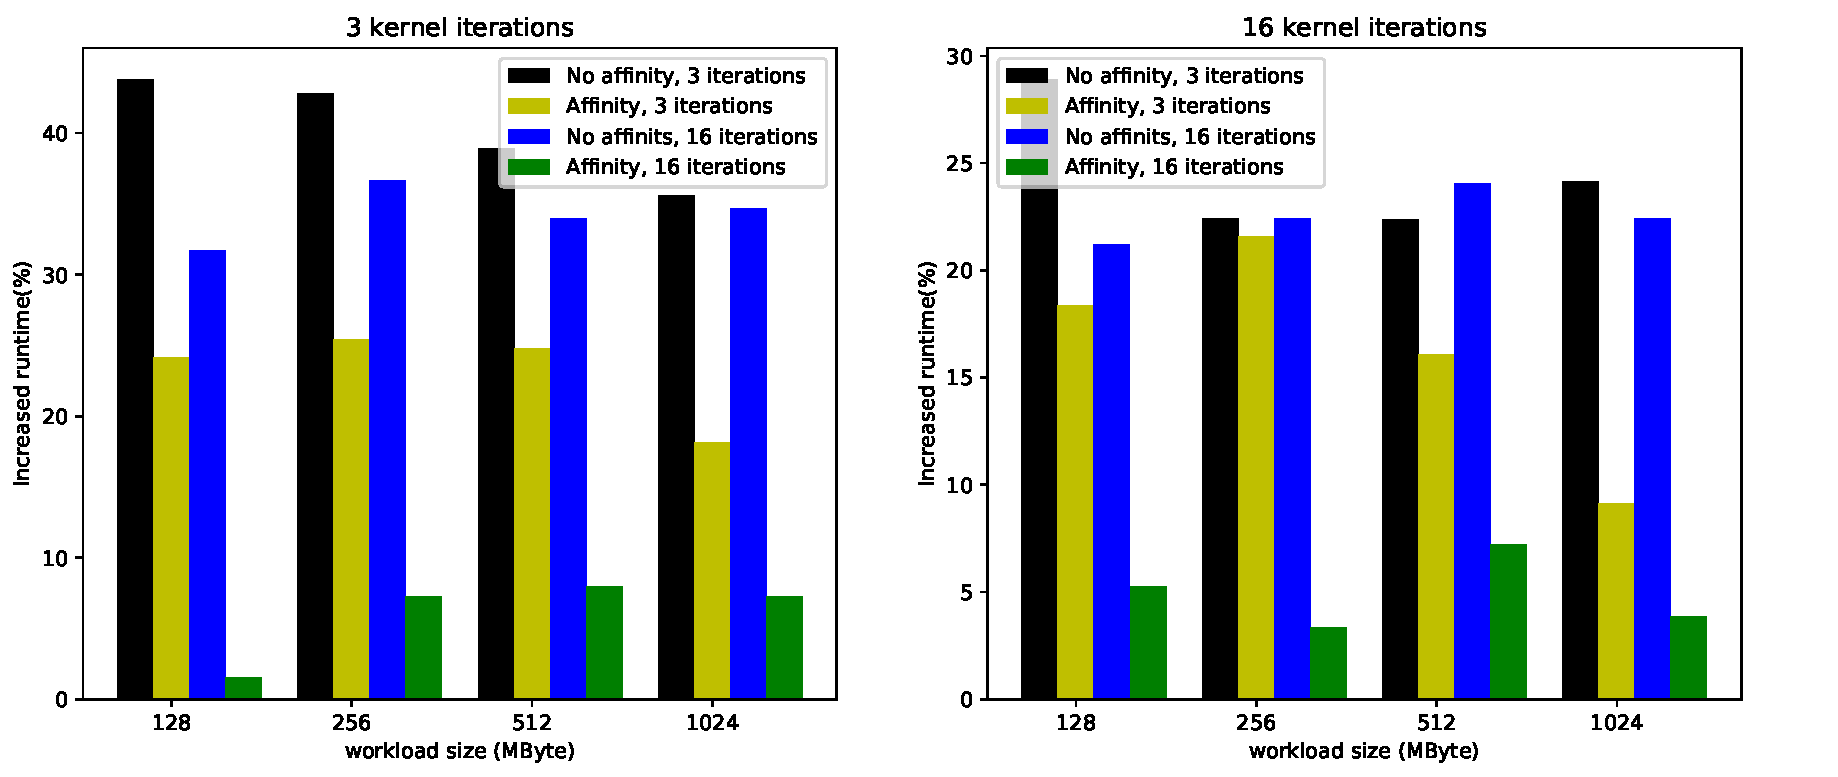
\includegraphics[width=\textwidth]{app-perf}
	\caption{ NUMA-Effects on pseudo-workload. Displayed as increase of runtime relative to a run with ideal NUMA placement between host and device. With implicit data movement.
		The left hand side shows the relative increase in short running computational kernels.
The right hand side shows the retlative increase on long computational kernels.}
	\label{f:apppref}
\end{figure}
For longer running kernels (16 kernel iterations) the data movement becomes less significant compared to compute time. Thus, the effects of NUMA locality are less visible in the data and the relative
performance overhead is reduced for all configurations, except the green one. It remains on its already
low level of overhead.

Figure\ref{f:apppref} shows the same experiment, but in this experiment data movement between host and device happend implicitly, using page-faults. The results show that the general assumptions about the data in \ref{f:appaff} still
hold true, however to smaller extend. This means that implicit data-movement creates a larger overhead, 
making NUMA effects less visible. In return this means that the explicit data movement benefits the overall
performance.
\begin{figure}
	\centering
	\begin{tabular}{|r|r|r|r|r|r|}
		\hline 
		Size [MByte] & Iterations & Kernel It. & Reference & Affinity & No Affinity\\ 
			\hline 
	128 & 3 & 3 & 251.25 & 353 & 636.5 \\ 
	\hline 
	128 & 3 & 16 &1328.75  & 1426 & 1936 \\ 
	\hline 
	128 & 16 & 3 & 429.5 & 525.25 & 584.25 \\ 
	\hline 
	128 & 16 & 16 & 2275.75 & 2354.5 & 2923.75 \\ 
	\hline 
	256 & 3 & 3 & 498.25 & 648.75 &  750.75\\ 
	\hline 
	256 & 3 & 16 & 2632 &2809.25  & 3801.5 \\ 
	\hline 
	256 & 16 & 3 & 876.5 & 998 & 1105.75 \\ 
	\hline 
	256 & 16 & 16 & 4367.25 & 4938.25 &5533.25  \\ 
	\hline 
	512 & 3 & 3 & 994 & 998 & 1429.75  \\ 
	\hline 
	512 & 3 & 16 & 5282.5 & 5583 & 7621 \\ 
	\hline 
	512 & 16 & 3 & 1701.25 & 1998.75 & 2172 \\ 
	\hline 
	512 & 16 & 16 & 8845 & 9237 & 10977.8 \\ 
	\hline 
	1024 & 3 & 3 &1958.25  & 2443.75  &2883.75 \\ 
	\hline 
	1024 & 3 & 16 & 10337 & 11054.8 &14645.5 \\ 
	\hline 
	1024 & 16 & 3 & 3336.5 & 3887.5 & 4292.25\\ 
	\hline 
	1024 & 16 & 16 & 17759.5  & 18078.2 & 22268.5\\ 
	\hline
	\end{tabular} 
	\label{tab:pref}
	\caption{Absolute Runtimes with Prefetch.}
\end{figure}
\begin{figure}
	\centering
	\begin{tabular}{|r|r|r|r|r|r|}
		\hline 
		Size [MByte] & Iterations & Kernel It. & Reference &  Affinity & No Affinity \\ 
		\hline 
	128 & 3 & 3 & 359.75 & 446.5 & 499.75 \\ 
	\hline 
	128 & 3 & 16 & 1918.5 & 1948.5 & 2507.75  \\ 
	\hline 
	128 & 16 & 3 & 534 & 632 & 683.25 \\ 
	\hline 
	128 & 16 & 16 & 2879.25 & 3031.25 & 3461 \\ 
	\hline 
	256 & 3 & 3 & 686 & 860.25 & 969 \\ 
	\hline 
	256 & 3 & 16 & 3684.5 & 3952.25 & 4939 \\ 
	\hline 
	256 & 16 & 3 & 1035.25 & 1258.75 & 1301.75 \\ 
	\hline 
	256 & 16 & 16 & 5584.5 & 5772.5 & 6606.25 \\ 
	\hline 
	512 & 3 & 3 & 1364 & 1702 & 1884.5 \\ 
	\hline 
	512 & 3 & 16 & 7209.25 & 7783 & 9883.5 \\ 
	\hline 
	512 & 16 & 3 & 2064.5 & 2396.5 & 2536.75  \\ 
	\hline 
	512 & 16 & 16 & 10868.2 & 11655 & 13499.5 \\ 
	\hline 
	1024 & 3 & 3 &2845.25  & 3361.75 &3693 \\ 
	\hline 
	1024 & 3 & 16 & 14395 & 15439 &19315 \\ 
	\hline 
	1024 & 16 & 3 & 4254 & 4641.5 & 5089\\ 
	\hline 
	1024 & 16 & 16 & 21778 & 22614.2 &26411.8 \\ 
	\hline
	\end{tabular}
	\label{tab:npref}
		\caption{Absolute Runtimes without Prefetch}
\end{figure}